\section{Evaluation}
\subsection{Experimental Setup}
\paragraph{Configurations} We evaluate \sysname on a single RTX-3090 with Qwen-8B (bf16). \sysname is implemented on SGLang with HiCache and chunked prefill~\cite{agrawal2024sarathi} enabled. For baseline comparison, we select vanilla SGLang and two opaque-request serving systems, CacheScout and Continuum~\cite{zhang2026cachescout, li2025continuum}.

\paragraph{Workloads.}
We evaluate \sysname using two representative agent applications: a fact-checking agent and a coding agent. Using these applications, we execute two benchmarks: HoVer~\cite{jiang2020hover}, a multi-hop fact verification benchmark requiring evidence collection and reasoning across multiple Wikipedia articles, and HumanEval~\cite{chen2021evaluating}, a code-generation benchmark that evaluates the functional correctness of generated programs using unit tests.
\subsection{Task quality and execution scale}
\sysname introduces prompt re-layout, which changes the ordering inside the prompt. Such a transformation should preserve comparable task quality and scale. As shown in Figure~\ref{fig:task-quality} and Table~\ref{tab:ablation}, all configurations achieve comparable task accuracy. At the same time, output tokens per session remain essentially the same. The observed serving improvements do not come at the cost of output quality or a reduction in task scale.

\begin{figure*}[t]
    \centering
    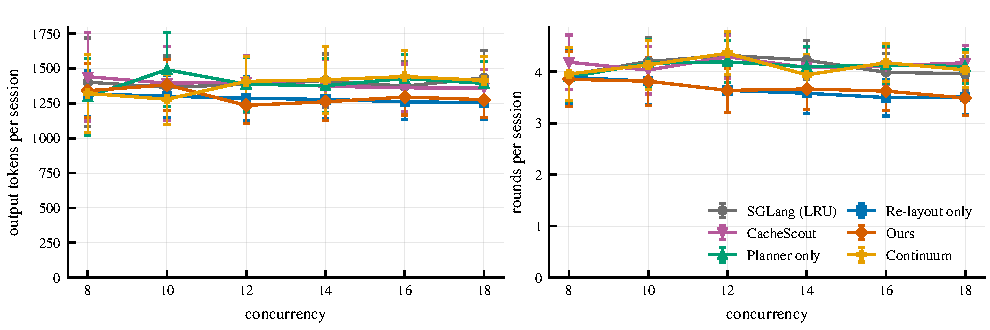
\includegraphics[width=1\linewidth]{figures/task_scale_fact.pdf}
    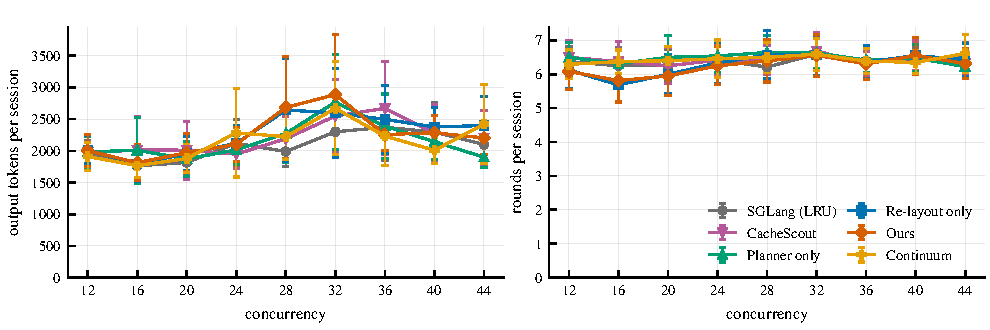
\includegraphics[width=1\linewidth]{figures/task_scale_code.pdf}
    \caption{Application-level task quality under varying concurrency for the
    HoVer fact-checking agent (left) and the HumanEval coding agent (right).}
    \label{fig:task-quality}
\end{figure*}

\begin{table}[t]
    \centering
    \caption{Application-level task quality across serving configurations.}
    \label{tab:ablation}
    \small
    \begin{tabular}{lcc}
        \toprule
        \textbf{Method}
        & \textbf{Fact Checking}
        & \textbf{Code Generation} \\
        \midrule
        SGLang (LRU)   & 57.2\% & 47.6\% \\
        CacheScout     & 57.2\% & 47.2\% \\
        Planner only   & 54.9\% & 46.2\% \\
        Re-layout only & 56.4\% & 45.5\% \\
        \textbf{Ours}  & \textbf{58.0\%} & \textbf{45.3\%} \\
        \bottomrule
    \end{tabular}
\end{table}
\subsection{Evaluation Analysis}
Our evaluations on \sysname address the following research questions:
\begin{enumerate}
    \item How much does \sysname improve end-to-end serving performance?
    \item How much do the two scheduling mechanisms of \sysname contribute to the improvement?
    \item How do the two mechanisms of heterogeneity-aware KV-cache scheduling in \sysname interact and reinforce each other?
\end{enumerate}
\subsubsection{RQ1: How \sysname improves end-to-end performance}
We evaluate \sysname on two representative agent applications: a fact-checking agent on the HoVer dataset and a coding agent on the HumanEval dataset. We use mean job completion time (JCT) and mean time to first token (TTFT) as the end-to-end performance metrics.

\paragraph{JCT}
As shown in Figures~\ref{fig:jct-coding}, \ref{fig:jct-fact}, \ref{fig:speedup-coding}, and~\ref{fig:speedup-fact}, \sysname consistently reduces mean JCT over the vanilla SGLang baseline, achieving $1.3\times$--$1.7\times$ speedup on the fact-check agent and $1.1\times$--$1.3\times$ on the coding agent. On the fact-check agent, Continuum performs comparably to SGLang at low concurrency but its advantage vanishes as load increases, whereas \sysname sustains its gains across all concurrency levels. On the coding agent, \sysname outperforms every other system; CacheScout and Continuum degrade sharply at high concurrency and fall behind SGLang.

\paragraph{TTFT}
\sysname also lowers mean TTFT across all workload configurations (Figures~\ref{fig:ttft-coding} and~\ref{fig:ttft-fact}). On the fact-check agent, the reduction is substantial at every concurrency level, while Continuum and CacheScout offer little or no improvement over SGLang. On the coding agent, \sysname matches or beats all baselines up to a concurrency of 40; at the highest concurrency, KV-only achieves a slightly lower TTFT.

\paragraph{Multi-Program serving of \sysname}
To understand how \sysname performs when serving multiple programs, we evaluate \sysname with a mixed workload of the fact-checking and coding agents sharing one server. We set concurrency at 16: 4 lanes consecutively launch fact-checking sessions and 12 lanes consecutively launch coding sessions, and all 16 lanes run in parallel. We select this 1:3 ratio based on the KV-cache footprint of the two agents. Every system first observes two sessions of each program, which are excluded from the numbers. We report throughput and mean TTFT for this evaluation. Throughput is calculated as the number of sessions completed per minute while all 16 lanes are busy.

Table~\ref{tab:multi-program} shows the results. The throughput of \sysname has a $1.51\times$ speedup over SGLang, with a mean TTFT speedup of $2.37\times$. Meanwhile, CacheScout and Continuum barely improve throughput over SGLang, with a $1.02\times$ speedup; their mean TTFT shows up to a $1.33\times$ speedup over SGLang. The ablation arms show the same pattern as in the single-program experiments. Re-layout alone accounts for most of the miss-rate reduction (58.3\%) and a $1.36\times$ throughput gain. The planner alone, which stays inert on a single coding workload, now delivers a $1.23\times$ gain with 5.5 points fewer misses. In a mixed pool, the eviction decision is between programs with different reuse patterns, which is exactly the decision the learned per-program model informs. 

The mix also tests whether the structure \sysname learns is per program. Under interleaving, \sysname's next-call prediction is correct for 89\% of the fact-checking calls and 80\% of the coding calls.

\begin{table*}[t]
    \centering
    \caption{Performance of \sysname and baselines on a mixed workload of fact-checking and coding agents. \sysname improves throughput by $1.51\times$ and reduces mean TTFT by 58\% over SGLang, with the KV-cache miss rate falling from 87.0\% to 56.7\%.}
    \label{tab:multi-program}
    \small
    \begin{tabular}{lcccccc}
        \toprule
        \textbf{Method}
        & \textbf{Throughput}
        & \textbf{Speedup}
        & \textbf{Mean TTFT}
        & \multicolumn{3}{c}{\textbf{KV-cache status}} \\
        & (sess/min) & & (ms) & device & host & miss \\
        \midrule
        SGLang (LRU)   & 3.64 & $1.00\times$ & 6266 & 10.5\% &  2.5\% & 87.0\% \\
        CacheScout     & 3.70 & $1.02\times$ & 4712 & 14.1\% &  2.3\% & 83.6\% \\
        Continuum      & 3.72 & $1.02\times$ & 4964 & 10.1\% &  4.5\% & 85.4\% \\
        Planner only   & 4.47 & $1.23\times$ & 4254 & 13.9\% &  4.6\% & 81.5\% \\
        Re-layout only & 4.95 & $1.36\times$ & 4164 & 19.2\% & 22.6\% & 58.3\% \\
        \textbf{Ours}  & \textbf{5.51} & $\mathbf{1.51\times}$ & \textbf{2642} & \textbf{31.3\%} & 12.0\% & \textbf{56.7\%} \\
        \bottomrule
    \end{tabular}
\end{table*}


\begin{figure*}[h]
    \centering
    \begin{subfigure}[b]{\textwidth}
        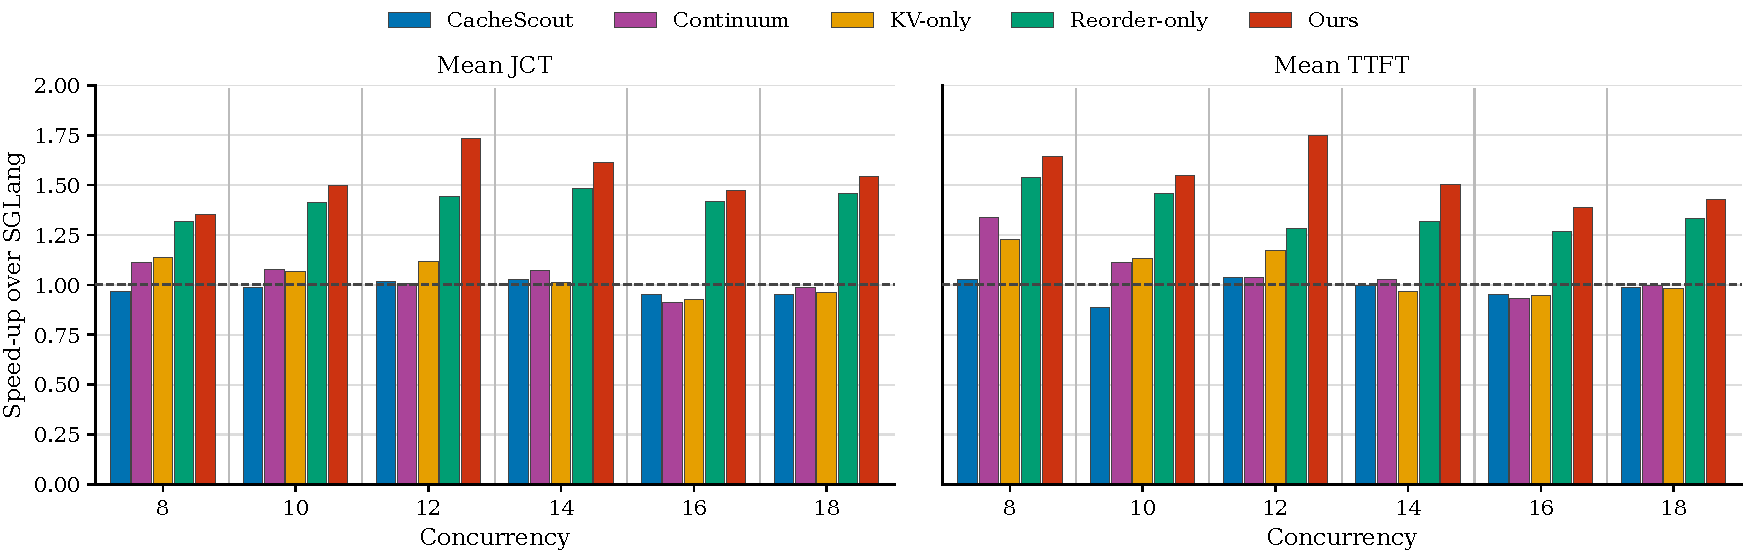
\includegraphics[width=\linewidth]{figures/speedup_fact.pdf}
        \caption{Fact Check Agent.}
        \label{fig:speedup-fact}
    \end{subfigure}
    \vspace{0.5em}
    \begin{subfigure}[b]{\textwidth}
        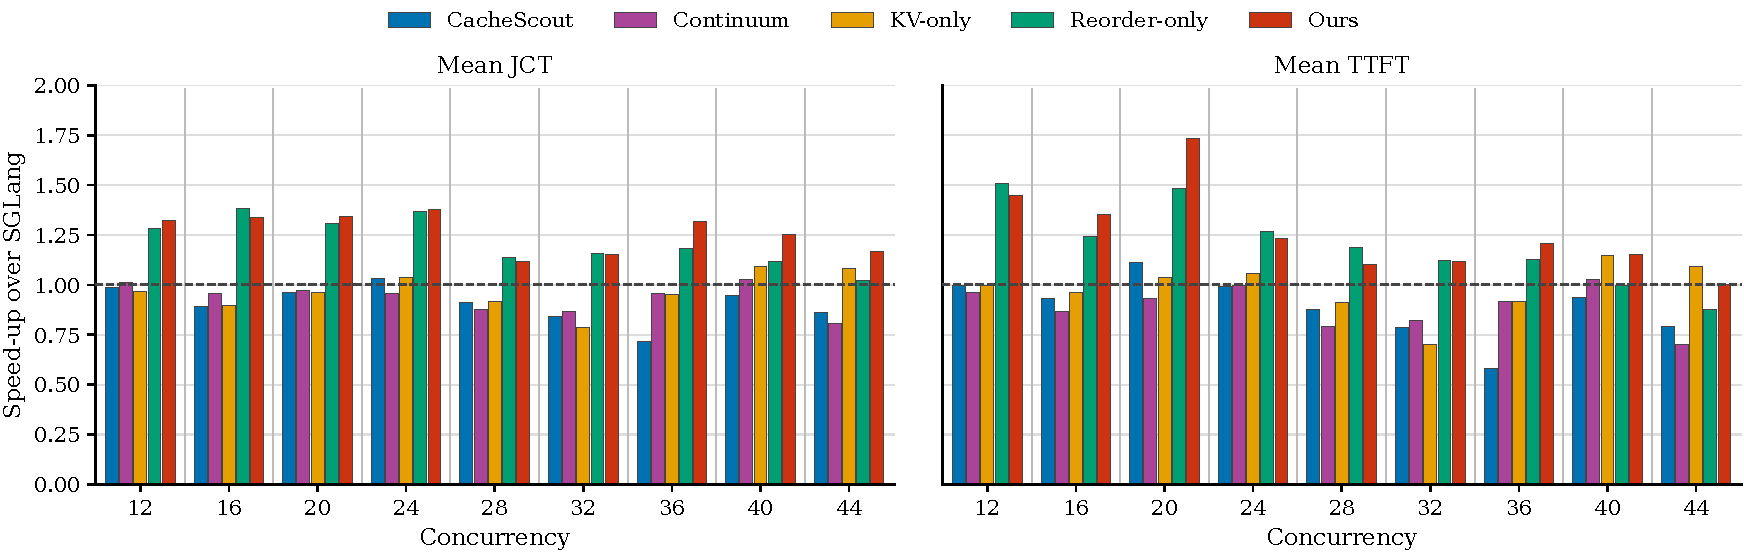
\includegraphics[width=\linewidth]{figures/speedup_coding.pdf}
        \caption{Coding Agent.}
        \label{fig:speedup-coding}
    \end{subfigure}
    \caption{Speed-up over SGLang in mean JCT and mean TTFT across concurrency levels.}
    \label{fig:serving-speedup}
\end{figure*}

\begin{figure}
    \centering
    \begin{subfigure}[b]{0.48\columnwidth}
        
\includegraphics[width=\linewidth]{figures/jct_coding.pdf}
        \caption{JCT: Coding.}
        \label{fig:jct-coding}
    \end{subfigure}\hfill
    \begin{subfigure}[b]{0.48\columnwidth}
        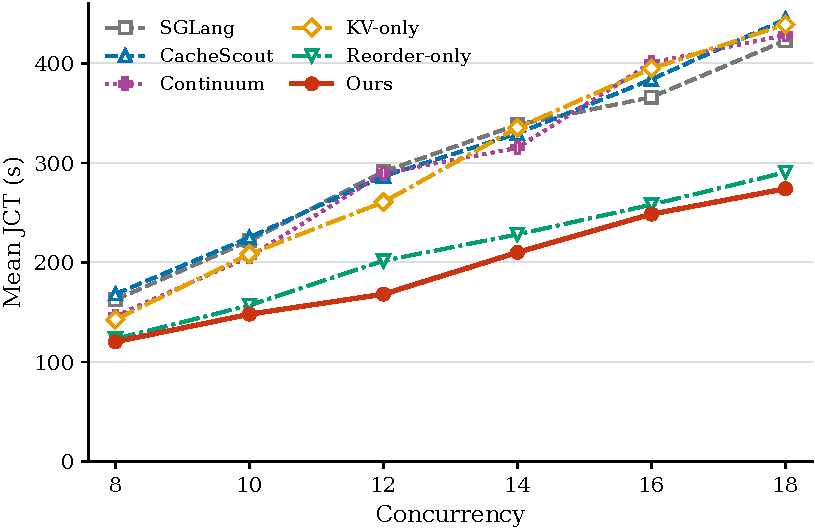
\includegraphics[width=\linewidth]{figures/jct_fact.pdf}
        \caption{JCT: Fact Check.}
        \label{fig:jct-fact}
    \end{subfigure}

    \vspace{0.4em}

    \begin{subfigure}[b]{0.48\columnwidth}
        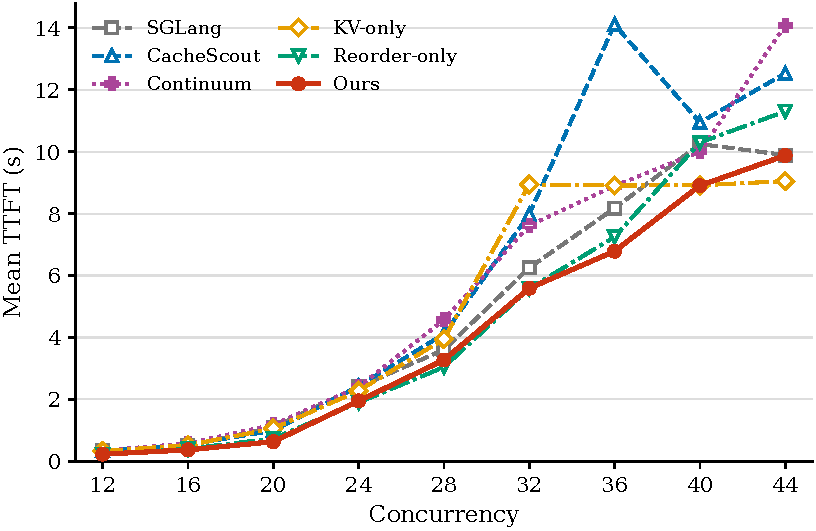
\includegraphics[width=\linewidth]{figures/ttft_coding.pdf}
        \caption{TTFT: Coding.}
        \label{fig:ttft-coding}
    \end{subfigure}\hfill
    \begin{subfigure}[b]{0.48\columnwidth}
        
\includegraphics[width=\linewidth]{figures/ttft_fact.pdf}
        \caption{TTFT: Fact Check.}
        \label{fig:ttft-fact}
    \end{subfigure}
    \caption{Mean JCT and TTFT across concurrency levels for the Coding Agent and Fact Check Agent.}
    \Description{Four line plots in a two-by-two grid comparing serving systems across concurrency levels: JCT and TTFT for the Coding Agent and Fact Check Agent.}
    \label{fig:serving-performance}
\end{figure}

\subsubsection{RQ2: How much the two scheduling mechanisms of \sysname contribute to the improvement}
\begin{figure}[h]
    \centering
    \begin{subfigure}[b]{\columnwidth}
        
\includegraphics[width=\linewidth]{figures/cache_coding.pdf}
        \caption{Coding Agent.}
        \label{fig:cache-coding}
    \end{subfigure}

    \vspace{0.5em}

    \begin{subfigure}[b]{\columnwidth}
        
\includegraphics[width=\linewidth]{figures/cache_fact.pdf}
        \caption{Fact Check Agent.}
        \label{fig:cache-fact}
    \end{subfigure}
    \caption{End-to-end KV-cache status (device hit, host hit, miss) under different concurrency levels.}
    \label{fig:cache-status}
\end{figure}
The improvement of \sysname comes from more efficient KV cache scheduling. From Figure~\ref{fig:cache-status}, it can be clearly observed that the performance gain comes from a lower KV cache miss rate. \sysname's heterogeneity-aware KV cache scheduling helps keep useful KV entries in cache. This scheduling mechanism incorporates two aspects, heterogeneity-aware prompt re-layout and prediction-guided KV management. We thus investigate detailed serving status to understand how the two KV scheduling mechanisms contribute to the performance improvement.

\paragraph{Speed-up introduced by heterogeneity-aware prompt re-layout}
To investigate the effects of prompt re-layout, we conduct an ablation experiment that disables \sysname's KV scheduling mechanism and uses only heterogeneity-aware prompt re-layout, shown as the \emph{re-layout only} arm in Figure~\ref{fig:cache-status}. When serving the coding agent, which is decode-heavy, re-layout obtains nearly all of the optimization when concurrency is below 28. But as the workload continues to grow, re-layout alone cannot sustain useful KV, the cache miss rate begins to drop, leading to a larger gap between it and full \sysname. Across sessions of the fact-check agent, re-layout only keeps a consistently slightly higher cache miss rate, which causes a performance deficit compared to full \sysname.

These evaluation results demonstrate that heterogeneity-aware prompt re-layout by itself helps enhance performance. Across all workload pressures, heterogeneity-aware prompt re-layout improves performance by introducing more opportunities for KV sharing, thus reducing cache misses and optimizing serving performance. It can even match full \sysname in some cases, but still falls behind full \sysname under high workload pressure.

\paragraph{Effects of Prediction-guided KV Management}
Adopting a similar methodology, we create an ablation arm that activates only the KV management of \sysname, which is the KV-only arm in Figure~\ref{fig:cache-status}. This mechanism shows substantially different behavior from prompt re-layout. In fact-check agent serving sessions, it only works under low pressure, where $c \le 14$, which is very similar to other KV management frameworks: Continuum and CacheScout also work only under very low concurrency levels. Moreover, this arm, together with Continuum and CacheScout, stays inert when serving the coding agent.

The reason for this phenomenon is straightforward: KV cache management needs space to operate. The effect of prediction-guided KV management comes from keeping useful entries in cache and preventing them from being evicted. However, when pressure is high, ongoing requests compete for memory and no KV cache can survive. Consequently, the effect of KV cache management diminishes under high workload pressure. A similar phenomenon can be observed for Continuum and CacheScout. But the effect of \sysname's prediction-guided KV management disappears much later than that of Continuum and CacheScout. On the fact-check agent, Continuum and CacheScout lose their effectiveness at $c=10$, while \sysname's prediction-guided KV management survives to $c=14$.

\subsubsection{RQ3: How the two mechanisms in \sysname's KV scheduling interact and reinforce each other}
\begin{figure*}[h]
    \centering
    \begin{subfigure}[b]{\textwidth}
        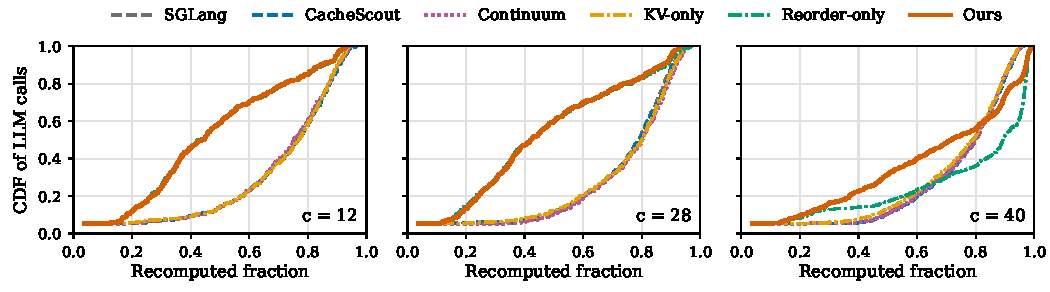
\includegraphics[width=\linewidth]{figures/recompute_cdf_coding.pdf}
        \caption{Coding Agent.}
        \label{fig:cdf-coding}
    \end{subfigure}

    \vspace{0.5em}

    \begin{subfigure}[b]{\textwidth}
        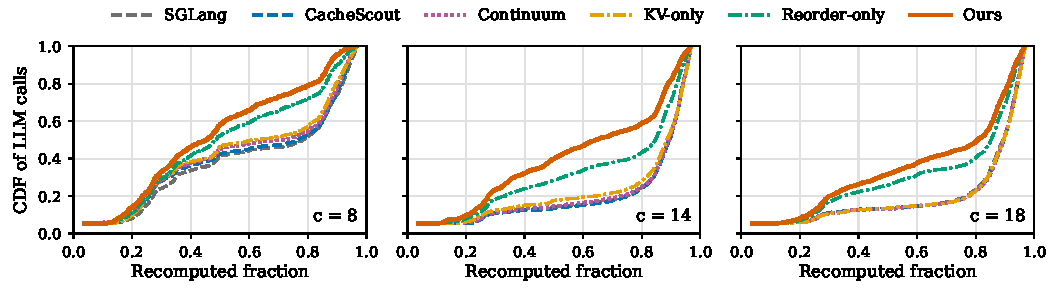
\includegraphics[width=\linewidth]{figures/recompute_cdf_fact.pdf}
        \caption{Fact Check Agent.}
        \label{fig:cdf-fact}
    \end{subfigure}
    \caption{CDF of the recomputed-token fraction per LLM call at representative concurrency levels.}
    \label{fig:recompute-cdf}
\end{figure*}
To analyze the interaction and mutual reinforcement of the two mechanisms, we scrutinize KV cache statistics and investigate some representative pressure points. We first analyze the behavior of \sysname under high workload.

When serving the coding agent, \emph{re-layout only} obtains the same performance as full \sysname. But under high workload pressure, full \sysname clearly works better: enabling \sysname's KV cache management mechanism further improves serving performance. Comparing the cache status in Figure~\ref{fig:cache-coding}, \emph{re-layout only} initially keeps the same cache miss rate (when $c \leq 28$) but its device miss rate increases, and the host tier catches the mistakenly evicted KV entries. The efficient host-to-device KV cache loading in SGLang fills the gap, so performance does not diverge at those points. When concurrency grows beyond 32, full \sysname begins to outperform \emph{re-layout only}: it has fewer cache misses, leading to better performance.

This behavior also emerges on the fact-check agent. As mentioned above, \sysname's KV management algorithm only works under low pressure, where $c \le 14$. Heterogeneity-aware prompt re-layout is effective across all pressures because it creates more KV sharing opportunities, which leaves space for KV scheduling. Therefore, heterogeneity-aware prompt re-layout and prediction-guided KV management are not two isolated mechanisms: prompt re-layout creates space, and KV management further improves cache efficiency.

We select some representative workload pressures and investigate how many tokens are recomputed. We choose $c=12, 28, 40$ for the coding agent and $c=8,14,18$ for the fact-check agent. As shown in Figure~\ref{fig:cdf-coding}, prompt re-layout maintains exactly the same number of recomputed tokens as full \sysname, but at $c=40$ things are different: re-layout only is left behind, and adding KV scheduling further reduces the recomputed tokens. In the regime of the fact-check agent, all KV scheduling mechanisms reduce the recomputed tokens; CacheScout, Continuum, and \sysname all enhance cache efficiency. Similarly, when the workload is high, \sysname's prediction-guided KV management can add optimization on top of heterogeneity-aware prompt re-layout, but KV scheduling by itself cannot take effect.
